\documentclass[tikz,border=3mm,multi=tikzpicture]{standalone}
\usepackage{tikz}
\usetikzlibrary{arrows.meta,positioning}
\begin{document}
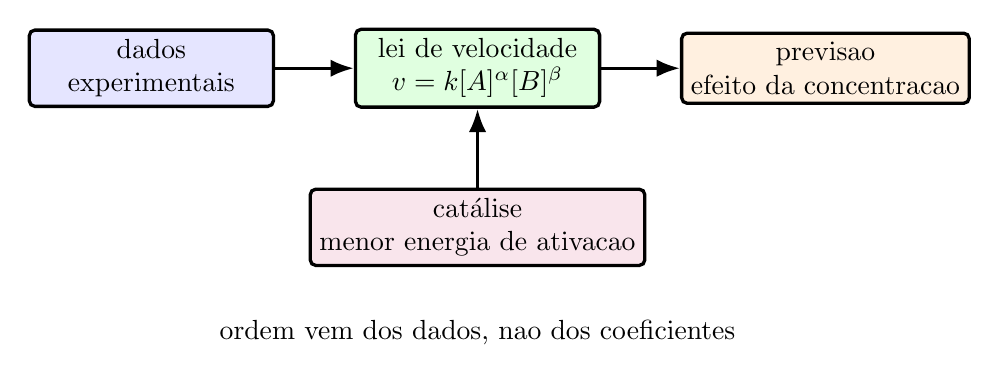
\begin{tikzpicture}[>=Latex,node distance=0.8cm]
  \tikzstyle{box}=[draw,rounded corners=2pt,very thick,minimum width=3.1cm,minimum height=0.85cm,align=center]
  \node[box,fill=blue!10] (dados) {dados\\experimentais};
  \node[box,fill=green!12,right=1cm of dados] (lei) {lei de velocidade\\$v=k[A]^\alpha[B]^\beta$};
  \node[box,fill=orange!12,right=1cm of lei] (prev) {previsao\\efeito da concentracao};
  \draw[very thick,->] (dados) -- (lei);
  \draw[very thick,->] (lei) -- (prev);
  \node[box,fill=purple!10,below=1.0cm of lei] (cat) {catálise\\menor energia de ativacao};
  \draw[very thick,->] (cat) -- (lei);
  \node[align=center,below=0.55cm of cat] {ordem vem dos dados, nao dos coeficientes};
\end{tikzpicture}
\end{document}
